\hypertarget{interfaceEnactable}{
\section{Enactable  Interface Reference}
\label{interfaceEnactable}\index{Enactable@{Enactable}}
}
Inheritance diagram for Enactable:\begin{figure}[H]
\begin{center}
\leavevmode
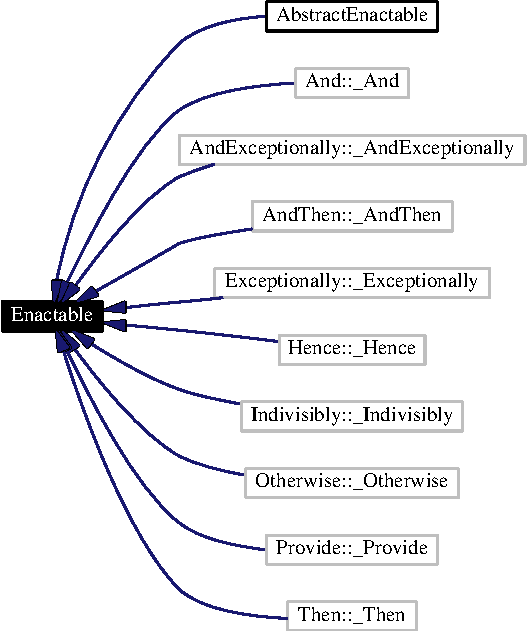
\includegraphics[width=144pt]{interfaceEnactable__inherit__graph}
\end{center}
\end{figure}
\subsection*{Public Methods}
\begin{CompactItemize}
\item 
\hyperlink{interfaceData}{Data} \hyperlink{interfaceEnactable_a0}{enact} (\hyperlink{interfaceData}{Data} data, \hyperlink{interfaceBindings}{Bindings} bindings) throws \hyperlink{classExceptional}{Exceptional}, \hyperlink{classFailed}{Failed}, \hyperlink{classUnfold}{Unfold}
\end{CompactItemize}


\subsection{Member Function Documentation}
\hypertarget{interfaceEnactable_a0}{
\index{Enactable@{Enactable}!enact@{enact}}
\index{enact@{enact}!Enactable@{Enactable}}
\subsubsection[enact]{\setlength{\rightskip}{0pt plus 5cm}\hyperlink{interfaceData}{Data} Enactable::enact (\hyperlink{interfaceData}{Data} {\em data}, \hyperlink{interfaceBindings}{Bindings} {\em bindings})}}
\label{interfaceEnactable_a0}




Referenced by Indivisibly::enact(), Hence::enact(), Otherwise::enact(), And\-Exceptionally::enact(), Exceptionally::enact(), And::enact(), And\-Then::enact(), Then::enact(), and Action\-Impl::enact().



The documentation for this interface was generated from the following file:\begin{CompactItemize}
\item 
\hyperlink{Enactable_8java-source}{Enactable.java}\end{CompactItemize}
